\subsection{Artificial Neural Networks}
\label{sub:ANN}

% Threshold Logic & Perceptron
In 1943, Warren S. McCulloch and Walter Pitts pioneered the concept of \glspl{nn} in their seminal paper \cite{mcculloch1943logical}, inspired by observations of the neurophysiology of the brain. In a simplified analogy, the brain can be thought of as a network of interconnected neurons, each consisting of a cell body (soma) and a nerve fibre (axon). These neurons communicate through synapses, where the axon of one neuron connects to the soma of another. The neuron transmits electrical impulses when its excitation exceeds a certain threshold.
\newline
\newline
In 1958, Frank Rosenblatt extended this neural network idea by introducing the perceptron model \citep{rosenblatt1958perceptron}. The perceptron serves as the basic unit of a neuron, with $n$ inputs and a single output. It contains multiple weights, a bias term, and an activation function. The core components and the process of computing an output are illustrated in Figure \ref{fig:Perceptron_Visualisation}.

\begin{figure}[htbp]
    \centering
    \begin{tikzpicture}
    
    \def\nodedist{45pt}
    \def\layerdist{70pt}
    \def\pindist{20pt}
    
    \tikzstyle{every pin edge}=[signal]
    \tikzstyle{annot} = [text width=4em, text centered]
    
    % input nodes
    \foreach \y in {1,...,3}
        \node[inputnode, pin={[pin edge={latex-}, pin distance=\pindist]left:Input \y}] 
            (x\y) at (0,-\y*\nodedist) {$x_\y$};
    
    % sum
    \node[infonode] 
            (sigma) at ($(x2) + (\layerdist, -0*\nodedist)$) {$\displaystyle\Sigma$};
            
    % bias
    \node[inputnode, label=above:{\parbox{2cm}{\centering Bias}}] at (sigma|-x1) (b1) {$b_1$};
    
    % activation function
    \node[infonode, label=above:{\parbox{2cm}{\centering Activation\\ function}}] 
            (activation) at ($(sigma) + (\layerdist, -0*\nodedist)$) {$f(z)$};
            
    % output node
    \node[outputnode, pin={[pin edge={-latex}, pin distance=\pindist]right:Output}]
            (output) at ($(activation) + (\layerdist, -0*\nodedist)$) {$\hat{y}$};
    
    % arrows 
    \draw[signal] (x1) -- (sigma) node [below right=0.25 and 0.05 of x1] {$\theta_{11}$};
    \draw[signal] (x2) -- (sigma) node [below right=-0.1 and 0.05 of x2] {$\theta_{12}$};
    \draw[signal] (x3) -- (sigma) node [below right=-0.5 and 0.05 of x3] {$\theta_{13}$};
    \draw[signal] (b1) -- (sigma);
    \draw[signal] (sigma) -- (activation);
    \draw[signal] (activation) -- (output);
    
    \end{tikzpicture}
    \caption{Visualisation of a perceptron.}
    \label{fig:Perceptron_Visualisation}
\end{figure}

\noindent
The inputs, denoted as $x_1, x_2, x_3 \in \mathbb{R}$, represent the values fed to the perceptron.\
These inputs are the basis for the following calculations.\
The weights $\theta_{11}, \theta_{12}, \theta_{13} \in \mathbb{R}$ are coefficients associated with each input.\
They determine the influence of each input on the perceptron's computation.\
The bias term $b_1 \in \mathbb{R}$ plays a special role as it acts like a weighted input but introduces an offset in the input space.\
And the activation function $f(z)$ is essential for introducing non-linearity in the perceptron's output.\
Without it, the \gls{nn} would only be able to represent linear functions.\
However, by introducing non-linearity through the activation function, a layered \gls{nn} with sufficient capacity can learn and approximate complex functions.\
Common activation functions include the sigmoid, the hyperbolic tangent \gls{tanh}, the rectified linear unit \gls{relu} and the softmax, as shown in the figure \ref{fig:Activation_Functions}.\
Each activation function has unique properties that make it suitable for specific tasks.
\newline
\newline
The output $a_i$ is the result of applying the activation function to the internal computation of the perceptron.\
This output is obtained using the equation \ref{eq:Perceptron-Calculate-Output}.\
In the context of a perceptron, $a_i$ represents the final output of the \gls{nn}.
\newline
\newline
It's important to note that the interpretation of the output $\hat{y}$ depends on the specific activation function used to compute it.\
The process of calculating the output of a neural network is called \textit{forward propagation}.

\myequations{Calculates the output of single layer neural network}
\begin{equation}
    \centering
    a_i = f(z_i) = f\Big(b_i + \sum_{j=1}^n \theta_{ij} \cdot x_j \Big) \text{ for } x_i, \theta_{ij}, b_i \in \mathbb{R}
    \label{eq:Perceptron-Calculate-Output}
\end{equation}

\begin{figure}[ht]
    \centering
    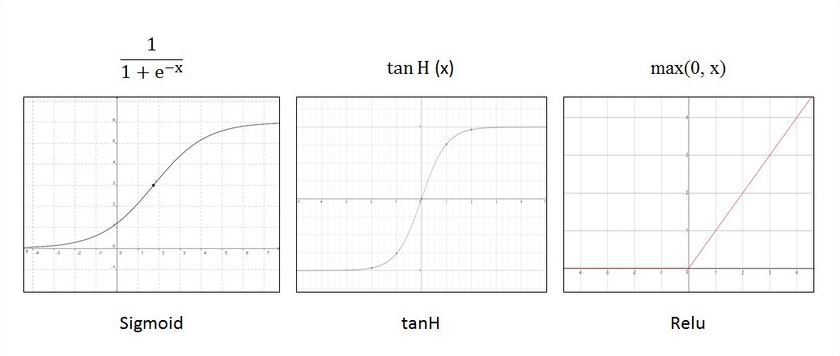
\includegraphics[width=1.0\textwidth]{./assets/img/activation_function.png}
    \caption{Figure shows the three activation functions sigmoid, tanh, and ReLu and their respective equation. Figure from \cite{haque2018image}}
    \label{fig:Activation_Functions}
\end{figure}

\noindent
% Multi-Layer Perceptron
Following the invention of the perceptron, researchers began to stack multiple perceptrons in layers and interconnect these layers.\
In this arrangement, the outputs of perceptrons in one layer serve as inputs to perceptrons in the next layer.\
This architecture is commonly known as a \gls{mlp}, as shown in Figure \ref{fig:MLP-Visualisation}.
\newline
\newline
The \gls{mlp} shown in Figure \ref{fig:MLP-Visualisation} consists of four different layers ($L$ = 4).\
The first layer is referred to as the \textit{input layer}, while the last layer is referred to as the \textit{output layer}.\
Intermediate layers between the input and output layers are commonly referred to as \textit{hidden layers}.
\newline
\newline
These hidden layers are often referred to as \textit{fully connected layers} because every input in one layer is connected to every perceptron in the next layer.\
This connectivity results in an extensive network of interconnected weights, allowing for complex data transformations and feature extraction.

\begin{figure}[htbp]
    \centering
    \begin{tikzpicture}[]
        \def\nodedist{35pt}
        \def\layerdist{80pt}
        \def\pindist{20pt}
        
        \tikzstyle{every pin edge}=[signal]
        \tikzstyle{annot} = [text width=4em, text centered]
        
        \foreach \y in {1,...,3}
            \node[inputnode, pin={[pin edge={latex-}, pin distance=\pindist]left:Input \y}] 
                (I\y) at (0,-\y*\nodedist) {$x_\y$};  
    
        \foreach \y in {1,...,4}
            \node[hiddennode] 
                (H1\y) at ($(\layerdist,-\y*\nodedist) +(0, 0.5*\nodedist)$) {$z_\y^1$};
        
        \foreach \y in {1,...,4}
            \node[hiddennode] 
                (H2\y) at ($(2*\layerdist,-\y*\nodedist) +(0, 0.5*\nodedist)$) {$z_\y^2$};
        
        \foreach \y in {1,...,2}
            \node[outputnode, pin={[pin edge={-latex}, pin distance=\pindist]right:Output \y}]
                (O\y) at ($(H21) + (\layerdist, -\y*\nodedist)$) {$\hat{y}_\y$};
    
        \foreach \dest in {1,...,4}
            \foreach \source in {1,...,3}
                \draw[signal] (I\source) -- (H1\dest);
        
        \foreach \dest in {1,...,4}
            \foreach \source in {1,...,4}
                \draw[signal] (H1\source) -- (H2\dest);
        
        \foreach \dest in {1,...,2}
            \foreach \source in {1,...,4}
                \draw[signal] (H2\source) edge (O\dest);
    
        \node[annot, above=4pt of H11] (hl) {Hidden layer 1};
        \node[annot, above=4pt of H21] (hl) {Hidden layer 2};
        \node[annot] at (I1 |- hl) {Input layer};
        \node[annot] at (O1 |- hl) {Output layer};
    \end{tikzpicture}
    \caption[Visualisation of a multilevel perceptron]{Visualisation of a multilevel perceptron, where $z_1^1$ is one example of a single perceptron in the network}
    \label{fig:MLP-Visualisation}
\end{figure}

\noindent
% Training Process
To obtain accurate results, the \gls{nn} must learn the optimal parameters $\theta_{ij}^{(l)}$ for a given problem.\
This learning process is facilitated by a technique known as backpropagation and optimisation.\
Backpropagation is an algorithm designed to determine how well the current predictions match the desired solution by computing gradients of the loss function with respect to the network parameters.\
The first step in backpropagation is to evaluate the discrepancy between the current predictions and the desired outcome.\
This evaluation is typically based on a loss function denoted as $\mathcal{L}$ or, in some contexts, a cost function.\
For regression tasks, the mean squared error (\gls{mse}) is often used and can be calculated using the equation \ref{eq:mean_squared_error}.\
Equation \ref{eq:cross-entropy} shows the calculation for the cross-entropy loss, which is often used in classification tasks.\
Having calculated the loss, the next step is to quantify the impact of each weight $\theta_{ij}^{(l)}$ on the error incurred.\
This is done by calculating gradients of the cost function $\mathcal{L}$ relative to the weights $\theta_{ij}^{(l)}$.\

\myequations{Mean Squared Error}
\begin{equation}
    \centering
    \mathcal{L}_{\text{MSE}}(y, \hat{y}) = \frac{1}{n} \sum^n_{i=1}(y_i - \hat{y}_i)^2
    \label{eq:mean_squared_error}
\end{equation}

\myequations{Cross-Entropy}
\begin{equation}
    \centering
    \mathcal{L}_{\text{CE}}(y, \hat{y}) = - \frac{1}{n} \sum^n_{i=1}\sum^K_{k=1}y_{ik} \cdot \text{log}(\hat{y}_{ik})
    \label{eq:cross-entropy}
\end{equation}

\noindent
The gradient serves as an indicator of both direction and rate, indicating the fastest ascent.\
The equation \ref{eq:backpropagation_gradient} calculates the gradients of the cost function $\mathcal{L}$ with respect to the weights $\theta_{ij}^{(l)}$ using partial derivatives.\
This equation is particularly focused on computing the gradients of the weights coming from the last hidden layer (\textit{hidden layer 2}, e.g. $z_1^2$) shown in figure \ref{fig:MLP-Visualisation}), where $l = 2$.\
For lower layers within the network, the chain rule of differentiation becomes more complicated and needs to be applied more extensively.\
Furthermore, the same mathematical framework can be used to compute the gradients of the cost function $\mathcal{L}$ with respect to the bias terms.\
Since the cost function doesn't depend directly on the weights, the chain rule becomes an essential tool for these calculations.

\myequations{Gradient of cost function with respect to the weights}
\begin{equation}
    \centering
    \frac{\partial \mathcal{L}}{\partial\theta_{ji}^{(l)}} = \frac{\partial \mathcal{L}}{\partial\hat{y}_i}\times\frac{\partial\hat{y}_i}{\partial z^{(l)}_j}\times\frac{\partial z^{(l)}_j}{\partial\theta_{ji}^{(l)}}
    \label{eq:backpropagation_gradient}
\end{equation}

\noindent
The final step in the learning process of a \gls{nn} is optimisation.\
In the equation \ref{eq:nn_optimisation}, the weights and biases are adjusted in proportion to the negated gradient of the cost function with respect to their respective weight or bias.\
This iterative learning process is repeated until the \gls{nn} converges to either a local or global minimum.\
To maximise the changes to find a global or local minima, a learning rate $\alpha$ that controls the step size is used. The learning rate controls the step size taken during the optimisation process, thus allowing a more efficient search for the optimal solution.

\myequations{Optimisation of the weights and biases}
\begin{equation}
    \centering
    \theta_{ij}^{(l)} \leftarrow \theta_{ij}^{(l)} - \alpha \nabla \mathcal{L}\Big(\theta_{ij}^{(l)}\Big) 
    \label{eq:nn_optimisation}
\end{equation}